\documentclass[11pt,a4paper]{article}

\usepackage[utf8]{inputenc}
\usepackage[T1]{fontenc}
\usepackage{amsmath,amssymb,amsthm}
\usepackage{mathtools}
\usepackage{graphicx}
\usepackage{float}
\usepackage{tikz}
\usepackage{tikz-cd}
\usetikzlibrary{arrows.meta,positioning,calc}
\usepackage[colorlinks=true,linkcolor=blue,citecolor=blue,urlcolor=blue]{hyperref}
\usepackage[margin=1in]{geometry}
\usepackage{xcolor}
\usepackage{listings}
\usepackage[numbers]{natbib}

% theorem environments
\theoremstyle{definition}
\newtheorem{definition}{Definition}[section]
\newtheorem{example}[definition]{Example}
\newtheorem{axiom}{Axiom}
\theoremstyle{plain}
\newtheorem{lemma}[definition]{Lemma}
\newtheorem{theorem}[definition]{Theorem}
\newtheorem{conjecture}[definition]{Conjecture}
\newtheorem{proposition}[definition]{Proposition}
\newtheorem{corollary}[definition]{Corollary}
\theoremstyle{remark}
\newtheorem{remark}[definition]{Remark}

% gap marker: every unfinished proof or missing piece is visible
\newcommand{\gap}[1]{\noindent\textcolor{red}{\textbf{[GAP: #1]}}}

% notation macros
\newcommand{\sset}{\mathsf{sSet}}
\newcommand{\causalO}[1]{\mathcal{C}_{\prec_\mathcal{H}}(#1)}
\newcommand{\Lin}{\mathcal{L}}
\newcommand{\colim}{\operatorname*{colim}}
\newcommand{\Cat}{\mathsf{Cat}}
\newcommand{\N}{\mathrm{N}}

\title{A Framework for Spacetime from Weighted Histories}
\author{Russi Chatterjee}
\date{\today}

\begin{document}

\maketitle

\begin{abstract}
We formulate a research framework for investigating whether spacetime and
quantum fields can arise from a common underlying structure. Candidate
histories are finite relational structures considered up to isomorphism.
Admissibility conditions specify which histories are possible, while a
separate weighting specifies how alternatives contribute to predictions.
To allow interference, the weighting is a strongly positive decoherence
functional rather than an ordinary probability distribution over individual
histories. Probabilities are assigned to decoherent families of alternatives.
This quantum structure is an assumption, not a derivation from combinatorics.
No external growth time is introduced. Physical time is instead a proposed
relation between internal clock readings and other records. The central
question is whether suitable admissibility conditions and weights support
effective geometry and matter dynamics that remain stable under changes in
microscopic details. A four-history quantum example makes the distinction
between admissibility, interference, and records explicit. It gives
phase-dependent output probabilities, a relation between record overlap
and fringe visibility, and a bound on the error of a diagonal approximation.
These are standard quantum calculations within the framework, not a
derivation of quantum mechanics or spacetime. A structural selection of the
weights, recovery of general relativity and quantum field theory, and
definition of a horizon entropy remain open.
\end{abstract}

% \tableofcontents

\section{Introduction}
\label{sec:introduction}

General relativity describes a dynamical spacetime geometry, while quantum
field theory describes quantum matter and its interactions on a specified
spacetime background. The aim of this work is to investigate a structure
from which both descriptions could be recovered in appropriate regimes.
The underlying objects need not themselves be points of spacetime, and
their mathematical description need not begin with a metric or an external
time parameter.

The proposal concerns a space of admissible histories together with weights
that determine how alternatives contribute to observations. A history is a
relational structure, not initially a trajectory through an already defined
space. Admissibility specifies which relations can coexist. Weighting is a
separate part of the model, since knowing which structures are possible does
not by itself determine their relative contributions. Quantum interference
requires more than an ordinary probability distribution over alternatives.
We therefore use a finite decoherence-functional description, drawing on
the histories-based treatment of quantum theory \citep{sorkin1994quantummeasure}.
This imports a quantum probability framework. It does not explain its origin.

The physical question is whether such a model can support persistent
organisation with a useful spacetime description. A successful account
would explain why the same effective laws survive a range of changes in
microscopic details. It would also have to distinguish structures that are
merely admissible from regimes that have appreciable probability within an
appropriate decoherent family. Neither persistence nor probability is
defined by resemblance to the physics one hopes to recover.

In this formulation there is no external process that traverses the space
of histories. A calculation that enumerates a history is not itself a
physical clock. Time would have to be recovered from correlations between
internal records, in the spirit of relational approaches
\citep{page1983}. This leaves the construction of clocks and the origin of
an arrow of time as separate problems. Likewise, cosmological expansion
would concern an effective metric relative to such clocks, not the number
of objects introduced by an enumeration algorithm.

Relational structures, histories, and inference principles already occur in
causal set theory \citep{bombelli1987,rideout2000csg,surya2019living},
rewriting approaches \citep{gorard2020}, and entropic dynamics
\citep{caticha2011}. These precedents do not establish the present proposal,
and no claim of novelty for these ingredients is made here. The required
comparison with those programmes remains part of the work.

To give the framework a concrete test, we specify four histories for a
two-path process and construct their weights from fixed mixing operations,
a phase, and an auxiliary route record. The model yields explicit output
probabilities, an interference visibility controlled by record overlap,
and an error bound for replacing coherent alternatives by a classical
mixture. The route and output questions separately decohere even when
their joint refinement does not. Detector uncertainty and record entropy
also differ. These calculations make the distinction between histories,
weights, and records observable within the toy model.

The example uses standard quantum mechanics. It does not explain why
quantum mechanics holds, and its relational paths are not an emergent
spacetime. Its role is to give the framework a finite instance with
explicit assumptions and consequences, rather than leave every part as an
unspecified construction.

This is a framework paper, not a derivation of a physical theory. The
methodology separates admissibility, quantum weighting, records, and
effective geometry so that assumptions in one part cannot be presented as
results of another. Section~\ref{sec:toyresults} gives the finite-model
predictions and Section~\ref{sec:discussion} states what could falsify the
prescription and what it leaves unexplained. No relational signature,
weighting law, or continuum limit is shown to reproduce general relativity
or quantum field theory.

\section{The framework}
\label{sec:framework}

\subsection{The object}

At any moment, the universe is a finite simplicial set.
Its edges are directed by the simplicial structure itself, since the face maps assign every edge a source vertex and a target vertex.
It begins as a single vertex $\Delta^0$ and it grows from there.

The object is pre-geometric.
It is not spacetime, and it is not a representation of a spacetime lying elsewhere.
It carries no metric, no dimension, and no manifold structure.
Everything geometric has to be recovered from it.
Statements about space are made in the framework's own combinatorial terms.

Throughout, \textbf{edge} means a non-degenerate $1$-simplex.
Every vertex $v$ carries the degenerate edge $s_0 v$ running from $v$ to itself, and these are never counted, never created by a move, and never part of a chain.

\subsubsection{Growing the Simplicial Set}

\begin{definition}[Horn, filled and unfilled]
\label{def:horn}
A \textbf{horn} in a simplicial set $X$ is a map $h : \Lambda^n_k \to X$ and not a subcomplex of $X$.
Two horns are the same only when they are the same map, so two embeddings with the same image count separately.
The horn is \textbf{filled} in $X$ when some map $\Delta^n \to X$ restricts along $\Lambda^n_k \hookrightarrow \Delta^n$ to $h$, and \textbf{unfilled} otherwise.
It is \textbf{inner} when $0 < k < n$.
\end{definition}

\begin{remark}[Why unfilled is about existence]
\label{rem:degenerate}
Definition~\ref{def:horn} asks whether a filler exists and not whether a fill event has supplied one.
The difference decides whether the set of available moves is finite.
Take an edge $f$ and the inner horn $\Lambda^2_1 \to X$ whose two edges are $f$ followed by the degenerate edge at the target of $f$.
The degenerate $2$-simplex $s_1 f$ restricts to that horn, so the horn is filled in every simplicial set containing $f$, and it is never offered as a move.
The horn whose two edges are the degenerate edge at the source of $f$ followed by $f$ is filled by $s_0 f$ in the same way.
Under the other reading every edge would immediately offer a horn against each of its degeneracies, each such fill would mint a parallel copy of an edge that already exists, and the copy would offer horns of its own.
The pool of available moves would be infinite from the first sprout onward.
\end{remark}

% the above need a figure for visual aid

\begin{definition}[Move]
\label{def:moves}

The simplicial set grows by two local, non-deleting \textbf{moves}, which are pushouts along the following two monomorphisms of finite simplicial sets, where $\hookrightarrow$ denotes an inclusion of one simplicial set into another:

\begin{enumerate}
  \item \textbf{Sprout:} the coface $d^1 : \Delta^0 \hookrightarrow \Delta^1$, including $\Delta^0$ as the source vertex.
        A sprout can happen at any vertex $v$ of the current state.
        Performing it attaches a fresh directed edge from $v$ to a new vertex.
  \item \textbf{Fill:} $\Lambda^n_k \hookrightarrow \Delta^n$ for $0<k<n$.
        A fill can happen at any unfilled inner horn in the sense of Definition~\ref{def:horn}.
        Performing it attaches the missing face and interior.
        Each horn may be filled at most once.
\end{enumerate}

\end{definition}

\begin{figure}[H]
  \centering
  % Sprout and fill on a growing directed simplicial set.
% Requires in the preamble:
%   \usepackage{tikz}
%   \usetikzlibrary{arrows.meta,positioning}
%   \usepackage{xcolor}
% Include with \input{figures/fig-sprout-fill}

\definecolor{hornclr}{RGB}{186,117,23}
\definecolor{compclr}{RGB}{15,110,86}
\definecolor{cellclr}{RGB}{83,74,183}

\begin{tikzpicture}[
  x=1cm, y=1cm,
  vtx/.style   ={circle, draw, fill=white, inner sep=0pt,
                  minimum size=5.4mm, font=\tiny},
  ed/.style    ={-{Stealth[length=1.8mm]}, semithick},
  hrn/.style   ={-{Stealth[length=1.8mm]}, line width=1.1pt, hornclr},
  cmp/.style   ={-{Stealth[length=1.8mm]}, semithick, compclr},
  mis/.style   ={-{Stealth[length=1.8mm]}, semithick, densely dashed, hornclr},
  lbl/.style   ={font=\tiny, inner sep=1pt},
  pcap/.style  ={font=\scriptsize, align=center, anchor=north}
]

  %% (a) sprout
  \begin{scope}[xshift=0cm]
    \node[vtx] (a0) at (0,0)      {$v_0$};
    \node[vtx] (a1) at (0.75,1.0) {$v_1$};
    \draw[ed] (a0) -- (a1);
    \node[pcap] at (0.75,-0.50) {(a) sprout};
  \end{scope}

  %% (b) inner horn
  \begin{scope}[xshift=2.5cm]
    \node[vtx] (b0) at (0,0)      {$v_0$};
    \node[vtx] (b1) at (0.75,1.0) {$v_1$};
    \node[vtx] (b2) at (1.5,0)    {$v_2$};
    \draw[hrn] (b0) -- (b1);
    \draw[hrn] (b1) -- (b2);
    \draw[mis] (b0) -- (b2);
    \node[lbl, hornclr] at (0.75,0.34) {$\Lambda^2_1$};
    \node[pcap] at (0.75,-0.50) {(b) inner horn};
  \end{scope}

  %% (c) fill
  \begin{scope}[xshift=5.0cm]
    \node[vtx] (c0) at (0,0)      {$v_0$};
    \node[vtx] (c1) at (0.75,1.0) {$v_1$};
    \node[vtx] (c2) at (1.5,0)    {$v_2$};
    \fill[compclr, opacity=0.16] (c0.center) -- (c1.center) -- (c2.center) -- cycle;
    \draw[ed]  (c0) -- (c1);
    \draw[ed]  (c1) -- (c2);
    \draw[cmp] (c0) -- (c2);
    \node[pcap] at (0.75,-0.50) {(c) fill};
  \end{scope}

  %% (d) second tier
  \begin{scope}[xshift=7.5cm]
    \node[vtx] (d0) at (0,0)      {$v_0$};
    \node[vtx] (d1) at (0.75,1.0) {$v_1$};
    \node[vtx] (d2) at (1.5,0)    {$v_2$};
    \node[vtx] (d3) at (2.25,1.0) {$v_3$};
    \fill[cellclr, opacity=0.14]
      (d0.center) -- (d1.center) -- (d3.center) -- (d2.center) -- cycle;
    \draw[ed]  (d0) -- (d1);
    \draw[ed]  (d1) -- (d2);
    \draw[ed]  (d2) -- (d3);
    \draw[cmp] (d0) -- (d2);
    \draw[cmp] (d1) -- (d3);
    \draw[cmp] (d0) .. controls (-0.28,1.75) and (1.48,2.15) .. (d3);
    \node[pcap] at (1.125,-0.50) {(d) second tier};
  \end{scope}

\end{tikzpicture}


  \caption{The two moves and what each of them adds. In (a) a vertex
  sprouts a fresh directed edge to a new vertex. After a second sprout,
  (b) shows the composable pair $v_0 \to v_1 \to v_2$ whose composite is
  absent, an unfilled inner horn $\Lambda^2_1$ (amber, missing edge
  dashed). In (c) the fill supplies the composite $v_0 \to v_2$ (green)
  together with the $2$-simplex witnessing it (shaded). Panel (d) shows the
  state after a third sprout and both first-tier fills. Two distinct
  horns now call for a composite from $v_0$ to $v_3$, one built from
  $v_0 \to v_1$ with $v_1 \to v_3$ and one from $v_0 \to v_2$ with
  $v_2 \to v_3$. Each fill mints its own composite, so $a$ and $b$ are
  parallel edges rather than a single shared one. Only once both are
  present does the inner horn $\Lambda^3_1$ exist, since its three faces
  already carry all six edges of $\Delta^3$. Filling it therefore adds a
  $2$-simplex and a $3$-simplex but no edge. Only inner horns are ever filled,
  so edge direction is never inverted and the limit object is a
  quasicategory.}
  \label{fig:sprout-fill}
\end{figure}

\begin{remark}[The sprout is a horn fill as well]
\label{rem:sproutishorn}
The two moves are one kind of operation.
The source vertex of $\Delta^1$ is the face opposite the target, which is the horn $\Lambda^1_0$, so the sprout is the pushout along $\Lambda^1_0 \hookrightarrow \Delta^1$.
The move set is therefore a set of horn inclusions throughout, consisting of one outer horn in dimension one together with every inner horn in dimension two and above.
Admitting this outer horn costs nothing, because $0 < k < 1$ has no solutions and both horns of $\Delta^1$ are outer, so no composition is made invertible by it.
The remaining dimension-one horn $\Lambda^1_1 \hookrightarrow \Delta^1$ would attach a fresh edge ending at an existing vertex.
It is not used here, and the question of whether it should be is deferred to Section~\ref{sec:kfold}, where its mirror-symmetric role in closing the move set under edge reversal is taken up alongside the $k$-fold moves.
\end{remark}

The initial object is a single vertex $\Delta^0$. At any moment the current state is a finite simplicial set, and the next move is chosen from the set of available moves, which is the disjoint union of all sprout sites and all unfilled inner horns.


Every vertex is created by exactly one sprout, which supplies its first incoming edge.
Every other incoming edge is a composite supplied by a fill.
So sprout edges and composite edges never mix.
A sprout creates a fresh vertex and attaches a directed edge to it.
The composite joins two vertices that already exist.


Sprouting attaches a cone along its base and inner-horn filling is an anodyne extension.
In both cases the inclusion of the old state into the new one is a weak homotopy equivalence, so no move changes the homotopy type.
In our case the homotopy type remains that of a point.

\begin{remark}[What conserving the homotopy type costs]
\label{rem:contractible}
A state that is contractible at every event has trivial homotopy invariants at every event.
No such invariant can therefore be an observable of the theory, at any stage and in any limit.
The whole of the physical content has to be carried by the directed structure and by the order of the events.
This is a commitment rather than a convenience, and it should be read alongside Remark~\ref{rem:treecost}, which describes what the directed structure is able to carry.
Section~\ref{sec:kfold} returns to this commitment with the tool that measures it: conserving the homotopy type is the statement that the homotopy ledger of Proposition~\ref{prop:ledger} reads zero at every event, and every departure from it is bought and paid for, one circle per unit of branching.
\end{remark}


Which moves add an edge is a combinatorial fact about horns.

\begin{lemma}[Which moves add edges]
\label{lem:edges}
A sprout adds exactly one edge, a fill in dimension two adds exactly one edge, and a fill in dimension three or above adds no edge.
\end{lemma}

\begin{proof}
A sprout attaches $\Delta^1$ along its source vertex, so it adds the one edge of $\Delta^1$.
An inner horn $\Lambda^n_k$ contains every face of $\Delta^n$ except the interior and the $k$-th $(n-1)$-face.
For $n = 2$ the missing face is itself an edge, the composite, and the fill adds exactly that edge.
For $n \geq 3$, an edge $\{i, j\}$ of $\Delta^n$ lies in the face opposite vertex $l$ for every $l \notin \{i, j\}$, and at least two such $l$ exist because $\Delta^n$ has at least four vertices.
The horn misses at most one face, so every edge of the attached $\Delta^n$ already lies in a face the horn contains, and the fill adds no edge.
\end{proof}

Fills in dimension three and above add only simplices that say existing paths agree.
So every chain is built out of edges, and nothing above dimension one can be part of a chain.
Whatever geometric and metric structure this model has is carried by the vertices, the edges, and the causal order between events.
Treat the edges as a multigraph.
If two fills each produce a composite, keep both as separate edges.
The number of parallel edges is a record of how many fills happened there.
The order says which events can affect which.
The edge counts say how much happened.
Both are needed, and neither replaces the other.

\begin{definition}[Rule]
\label{def:rule}
The \textbf{rule} of an event is a specification that contains three pieces of information:
\begin{enumerate}
  \item \textbf{Find}: Which spots in the current simplicial set qualify for the move to happen.
  \item \textbf{Match}: Which spot the move is applied to.
  \item \textbf{Apply}: What new simplices the move puts in there.
\end{enumerate}
Formally, the rule is an inclusion $F \hookrightarrow A$ of finite simplicial sets, from the \textbf{find pattern} $F$ to the \textbf{apply pattern} $A$.
The match is an injective map $m_e : F \hookrightarrow X_{<e}$ from the find pattern into the state of the events strictly preceding $e$ (Definition~\ref{def:state}), and apply is the pushout of the rule along the match.
Injectivity forbids folded spots, where two simplices of the pattern land on the same simplex of the state.
The event adds the simplices of $A$ not in the image of $F$.
The find and apply patterns of an event $e$ are written $F_e$ and $A_e$.
\end{definition}

Three kinds of rules exist:

\begin{itemize}
  \item \textbf{The big bang.}
    Find: nothing needs to be found.
    Match: there is no spot to choose.
    Apply: the initial vertex $\Delta^0$ is created out of nothing ($\varnothing \hookrightarrow \Delta^0$).
  \item \textbf{A sprout.}
    Find: every vertex qualifies.
    Match: the chosen vertex $v$, a map $\Delta^0 \to X_{<e}$.
    Apply: attach $\Delta^1$ by its source vertex (the coface $d^1 : \Delta^0 \hookrightarrow \Delta^1$), adding an edge from $v$ to a fresh vertex.
  \item \textbf{A fill.}
    Find: every unfilled inner horn $\Lambda^n_k$ with $0 < k < n$ qualifies.
    Match: the chosen horn, an embedded copy of $\Lambda^n_k$ in $X_{<e}$.
    Apply: attach $\Delta^n$ along the horn ($\Lambda^n_k \hookrightarrow \Delta^n$), adding the missing face and the interior.
\end{itemize}

% TODO: or what if we have a more structured condition such that 2-level growth cannot happen or growth happens only on the edges and hence the internal sset must be complete first - but it will impose a very important global condition on spacetime! (or will it, i mean it will still be a local condition followed globally?)
% \begin{remark}[The quasicategory limit needs a fairness condition]
% \label{rem:fairness}
% The limit of the filling process is a quasicategory exactly when every inner horn is filled at some point.
% A history can fail this and still satisfy every condition imposed here.
% Each fill creates simplices that offer further horns, so the pool of unfilled inner horns grows as the history runs, and a rule may leave a given horn unchosen forever.
% Call a history \textbf{fair} when every inner horn of every state is filled at some later event.
% The limit of a fair history is a quasicategory.
% Fairness is a condition on the rule, it is not implied by anything else stated here, and it therefore belongs among the constraints on the inference problem rather than among the consequences of the move set.
% \end{remark}

\begin{remark}[The at-most-once convention]
\label{rem:atmostonce}
The last clause of Definition~\ref{def:moves} is automatic under the fill rule as stated, since the find pattern offers only unfilled inner horns, and a horn, once filled, is never offered again.
The clause is kept because it records a choice.
The alternative convention lets a filled horn be filled again, so that one horn can supply several witnesses to the same composite.
That variant changes what the events record, and with it any entropy built from the event record.
It is not studied here.
It is worth noting what is being set aside.
Under the refilling convention the number of composites between a fixed pair of vertices becomes an unbounded local quantity attached to that pair.
That is the only quantity anywhere in the framework which behaves like an edge length or a local volume, so the discarded variant is the one in which a metric variable could be carried.
\end{remark}
% hey but can we not say that for e.g. the simplex angles etc still hold a lot of metricizability in the way they are connected?

\subsection{History, runs, and the causal order}

Growth happens one move at a time.
The universe at any moment is a finite stage of an ongoing history, and each event after the big bang is a move applied at a particular spot.
Since no move deletes anything, an event can only apply to simplices that already exist.
Event $b$ therefore depends on event $a$ when the spot at which $b$ is applied contains, among its maximal simplices, one created by $a$, where a simplex of the spot is maximal when it is not a face of another simplex of the spot.
For a sprout the spot is a single vertex, which is maximal.
For a fill the maximal simplices of the horn $\Lambda^n_k$ are its $(n-1)$-faces, so a dimension-two fill depends on the two events that created the edges of its horn and not directly on the events that created its vertices.
The vertex creators still lie in the causal past by transitivity, since a simplex is only ever created after its vertices already exist.
The causal order of an event $e$ is the set of events that $e$ depends on directly or via other events, together with $e$ itself, with the order among them.
A reference frame is a linear extension of this order \citep{davey2002lattices}.

\begin{definition}[History]
\label{def:history}
A \textbf{history} $\mathcal{H}$ is a set of events carrying a strict partial order $\prec$ with a least element $\bot$, in which every event has only finitely many events below it, together with a rule and a match assigned to each event.
\end{definition}

The order is well founded and the strict pasts are finite, so the following is defined by recursion on $\prec$.
For each event $e$, the \textbf{state of the strict past}, written $X_{<e}$, is the simplicial set built by the events strictly below $e$, each of which is already available because its own strict past is smaller.
Every simplex of $X_{<e}$ is attached by exactly one of those events, and we write $\varepsilon(\sigma)$ for it.
The conditions are these.

\begin{enumerate}
  \item The least event $\bot$ carries the rule $\varnothing \hookrightarrow \Delta^0$, so it creates the initial vertex.
  \item Every other event $e$ carries a sprout or fill rule $F_e \hookrightarrow A_e$ together with an injective match $m_e : F_e \to X_{<e}$.
  \item Write $a \vartriangleleft e$ when $a = \varepsilon(\sigma)$ for some maximal simplex $\sigma$ of the image of $m_e$. Then $\prec$ is the transitive closure of $\vartriangleleft$.
\end{enumerate}


\begin{remark}[What the recursion fixes and what it does not]
\label{rem:recursion}
The earlier form of this definition described each event as applied to the simplicial set built by the events strictly preceding it, and left that simplicial set to be constructed in Definition~\ref{def:state}, which in turn needed the causal order, which needed the matches.
The recursion above removes the forward reference.
The order is posited first, well-foundedness makes the recursion legitimate, the states of the strict pasts are produced by it, and the third condition is then a check on the posited order rather than a definition of it.
What remains open is the stronger presentation in which no order is posited at all and events arrive as a bare family whose order is derived.
That presentation is the one that matches the claim that history is primary and the state is derived, and it is not developed here.
\end{remark}

A history maintains a record of every event and all of its data, namely its rule.
Different histories can result in the same simplicial set.
Nothing in the framework as stated selects one history over another, and we do not treat the collection of all histories as a single mathematical object here.
What selects the realized history is left open.
Posing that selection as a well-formed inference problem is one of the aims of this work.

\begin{definition}[Causal Order]
\label{def:causalorder}
A \textbf{causal order} $\causalO{e}$ of a history $\mathcal{H}$ for an event $e$ is the set of events preceding and including $e$, partially ordered by $\prec$, where $a \prec b$ if and only if $b$ depends on $a$ directly or via other events. Direct dependency is witnessed only by the maximal simplices of the spot, as fixed above, so a fill depends directly on the creators of the faces of its horn and only indirectly on the creators of its vertices. The \textbf{causal past} of $e$ is the causal order with $e$ itself removed.
\end{definition}

Every vertex is created by a unique event, the big bang for the initial vertex and a sprout for every other one, and we write $\varepsilon(v)$ for that event.
For every vertex $w$ other than the initial one we write $\pi(w)$ for the source of the sprout edge that created $w$, and call $\pi(w)$ the \textbf{parent} of $w$.
Call $u$ an \textbf{ancestor} of $w$ when $u$ is reached from $w$ by applying $\pi$ one or more times.

\begin{lemma}[Acyclicity of the one-skeleton]
\label{lem:acyclic}
The directed multigraph formed by the vertices and the non-degenerate edges of the state at any event has no directed cycles.
Degenerate edges have to be excluded, since $s_0 v$ is a loop at every vertex $v$.
\end{lemma}

\begin{proof}
The proof uses a single invariant, maintained by induction on events: every edge added by every move either has a vertex that is fresh at that move, or runs parallel to a directed path that already exists.
A sprout adds an edge into a fresh vertex, so it satisfies the invariant through freshness and cannot lie on a directed cycle, since a fresh vertex has no outgoing edges.
A fill adds no new vertices.
A dimension-two fill adds its composite parallel to the two-edge path supplied by its horn, satisfying the invariant directly; if that composite closed a directed cycle, the cycle minus the composite would be a directed path from target back to source in the previous state, which the induction hypothesis forbids.
A fill in dimension three or above adds no edges by Lemma~\ref{lem:edges}.
No move ever adds an edge between two pre-existing vertices other than such a composite, so no cycle is ever completed, and the induction runs along any linear extension of the history.
Note that the invariant and the argument never mention the causal order: acyclicity is a consequence of the shape of the moves alone, not of when they are applied.
This matters in Section~\ref{sec:kfold}, where moves are admitted whose edges violate the creator-precedes-created relation used in earlier drafts of this proof but satisfy the present invariant unchanged.
\end{proof}

\begin{proposition}[Reachability is the ancestor relation of a forest]
\label{prop:tree}
For every state and every edge $u \to w$, the vertex $u$ is an ancestor of $w$.
Consequently a directed path runs from $u$ to $w$ if and only if $u$ is an ancestor of $w$.
\end{proposition}

\begin{proof}
Induct along the causal order, as in Lemma~\ref{lem:acyclic}.
A sprout edge runs from an existing vertex $u$ to the fresh vertex $w$ it creates, and $\pi(w) = u$ holds by the definition of $\pi$, so $u$ is an ancestor of $w$.
A composite edge $u \to w$ is supplied by a fill whose horn carries edges $u \to v$ and $v \to w$, both created earlier.
The induction hypothesis makes $u$ an ancestor of $v$ and $v$ an ancestor of $w$, and the ancestor relation is transitive because it is the transitive closure of $\pi$.
By Lemma~\ref{lem:edges} there are no other edges.
For the second statement, every edge realises an ancestor relation and therefore so does every directed path, while conversely the sprout edges alone already join every vertex to each of its ancestors.
\end{proof}

\begin{corollary}[Incomparable vertices have no common future]
\label{cor:nocommonfuture}
Let $u$ and $w$ be vertices of a state with neither an ancestor of the other.
Then no vertex is reachable from both, at this event or at any later one.
\end{corollary}

\begin{proof}
Every vertex other than the initial one has exactly one parent, so the ancestors of a vertex $x$ are $\pi(x)$, then $\pi(\pi(x))$, and so on, which is a chain under the ancestor relation.
If some $x$ were reachable from both $u$ and $w$, then Proposition~\ref{prop:tree} would place $u$ and $w$ in that chain, making them comparable, against the assumption.
No move alters $\pi$ at a vertex that already exists, and no move removes a vertex, so the same argument applies at every later state.
\end{proof}

\begin{remark}[What Corollary~\ref{cor:nocommonfuture} costs]
\label{rem:treecost}
The reachability relation on vertices is the ancestor relation of a rooted tree.
This follows from the move set of Definition~\ref{def:moves} alone and not from any particular rule, so no choice of rule and no solution of the inference problem can change it.
Two consequences are worth stating plainly.
The causal past of a vertex is a chain, so it is one-dimensional as an order.
Two vertices that are not causally comparable share no future event, whereas in a Lorentzian manifold of dimension two or more any two spacelike separated points have points in their common causal future.
The framework as stated therefore offers no place for a spatial separation to live.
The only number the one-skeleton attaches to a pair of vertices is the multiplicity of parallel composites between them, and that number is defined only when the pair is already comparable.
Section~\ref{sec:kfold} sets out the smallest change to the move set that removes the obstruction, together with what the change costs.
\end{remark}

\begin{definition}[Run]
\label{def:run}
The \textbf{run} at event $e$, written $\mathcal{R}(e)$, is the subposet of $\causalO{e}$ consisting of the big bang and the events that add an edge, with the induced order. By Lemma~\ref{lem:edges} these are exactly the sprouts and the dimension-two fills.
\end{definition}

The run is closed downward.
A sprout depends only on the event that created its vertex, and vertices are created only by sprouts.
A dimension-two fill depends only on the events that created the two edges of its horn, and edges are created only by sprouts and dimension-two fills.
So no edge-adding event ever depends on a higher fill, and the run at $e$ is a downset \citep{davey2002lattices} of the history.
A general downset of the history is not a run: downsets may contain higher fills, while the run keeps only the edge-adding events.
The induced order is automatically a partial order, since a partial order restricted to a subset is still a partial order.
Moreover, the run at $e$ is a history in its own right, since it satisfies the three conditions:

\begin{enumerate}
  \item Every event of the run has only finitely many events below it in the history, hence also in the run.
  \item The big bang is included by definition and stays the least event.
  \item The induced order on the run is generated by creation-before-use. A sprout depends only on the event that created its vertex, which is a sprout, and a dimension-two fill depends only on the events that created the two edges of its horn, which are sprouts or dimension-two fills. So every direct dependency of an edge-adding event is again an edge-adding event, and dependency chains between run events never leave the run.
\end{enumerate}

At any moment, the run is the partially ordered record of exactly those events that change the one-skeleton.
It determines the one-skeleton of the state as a multigraph, with parallel composites kept distinct, and it forgets the higher fills entirely.
Passing from a history to its run forgets the higher fills, and passing from a run to its one-skeleton forgets the order.
Different histories can produce the same run, since higher fills leave no trace in it.
Different runs can produce the same one-skeleton, since the multigraph forgets the order.
Everything metric in this framework will be a function of the run, while the entropy of an event is a function of its causal order, which remembers the higher fills that the run forgets.

\begin{definition}[Entropy]
\label{def:entropy}
For a finite poset $P$, write $\Lin(P)$ for its set of linear extensions.
The \textbf{entropy} of an event $e$ is
\[
S(e) = \log |\Lin(\causalO{e})|,
\]
the logarithm of the number of linear extensions of the causal order.
The event $e$ is the unique maximum of $\causalO{e}$, so the causal past of $e$ has the same number of linear extensions, and the entropy measures how much of the past could have happened in a different order.
Logarithms are natural throughout.
\end{definition}

\begin{proposition}[Which events carry no entropy]
\label{prop:zeroentropy}
$S(e) = 0$ in each of these two cases.
\begin{enumerate}
  \item $e$ is the big bang or a sprout.
  \item $e$ is a dimension-two fill whose horn carries two sprout edges.
\end{enumerate}
\end{proposition}

\begin{proof}
A finite poset has exactly one linear extension when it is a chain, so it is enough to show that $\causalO{e}$ is a chain in both cases.
For the first case, a sprout at a vertex $v$ depends directly on the one event $\varepsilon(v)$ that created $v$, and $\varepsilon(v)$ is the big bang or a sprout, so the same holds of it.
Iterating reaches the big bang after finitely many steps, by the first condition of Definition~\ref{def:history}, and the causal order is the chain this produces.
For the second case, let the horn carry the sprout edges $u \to v$ and $v \to w$.
The second of these created $w$, so its creating event is $\varepsilon(w)$, a sprout applied at $v$, whose one direct dependency is $\varepsilon(v)$.
The first edge created $v$, so its creating event is $\varepsilon(v)$.
The two events the fill depends on are therefore comparable, each has a chain for its causal order by the first case, and the fill sits above both.
\end{proof}

\begin{remark}[What the entropy is measuring]
\label{rem:whatentropymeasures}
Proposition~\ref{prop:zeroentropy} says that fresh vertices and first-tier composites are free.
An event carries positive entropy only when it composes something that is itself a composite, which is what happens at the event $g$ of Example~\ref{ex:run}, whose horn carries the composite supplied by $f$ alongside a sprout edge.
So $S$ counts how deeply composition has been nested in the causal past, and not how much of the universe has been built.
Whatever second law the framework supports is a statement about the growth of the coherence tower, and the prose should not let it be read as a statement about the growth of space.
\end{remark}

\begin{remark}[The entropy is not a function of the geometric data]
\label{rem:notafunctionofrun}
Passing from a history to its run forgets the higher fills and the entropy of an event does not.
Two histories with the same run can therefore differ in $S$, since a dimension-three fill can be inserted into one of them and not the other while leaving both runs equal.
An area law is an equality between an entropy and a geometric quantity.
If everything geometric is a function of the run, as stated above, no such equality can hold for $S$ as it is defined here.
There are two ways out.
Either the entropy is rebuilt from the run alone, which gives up the nesting that Remark~\ref{rem:whatentropymeasures} identifies as its content, or the geometric data is enlarged until it sees the higher fills.
This has to be settled before a horizon computation can be posed at all.
\end{remark}

\begin{remark}[The entropy alone cannot select a causal structure]
\label{rem:antichain}
For posets on $n$ elements, $|\Lin(P)| \leq n!$ with equality exactly when $P$ is an antichain.
An inference principle that maximises $S$ under no further constraint therefore selects the causal order with no relations in it.
The same difficulty is known in causal set theory, where the uniform measure on $n$-element posets concentrates on the three-layer orders of \citet{kleitman1975}, which are not manifold-like, and where an action is introduced to suppress them \citep{surya2019living, loomis2018suppression}.
The constraint set for the maximum entropy problem has to do that work here as well.
Saying which constraint does it is a prerequisite for posing the problem and not a detail of solving it.
\end{remark}

\begin{example}
\label{ex:run}
Start from the single vertex $v_0$, created by the big bang.
The history grows by the following events.
\begin{enumerate}
  \item $s_1$: sprout an edge $v_0 \to v_1$.
  \item $s_2$: sprout an edge $v_1 \to v_2$.
  \item $s_3$: sprout a second edge $v_0 \to v_3$ from the starting vertex.
  \item $f$: fill the horn $v_0 \to v_1 \to v_2$, supplying the composite $v_0 \to v_2$ and its witnessing $2$-simplex.
  \item $s_4$: sprout an edge $v_2 \to v_4$.
  \item $g$: fill the horn $v_0 \to v_2 \to v_4$, whose first edge is the composite from $f$, supplying the composite $v_0 \to v_4$.
  \item $f'$: fill the horn $v_1 \to v_2 \to v_4$, supplying the composite $v_1 \to v_4$.
        Now all six edges among $v_0, v_1, v_2, v_4$ exist, and three of the four triangular faces carry $2$-simplices.
  \item $h$: fill the resulting inner horn $\Lambda^3_2$, supplying the missing face $(v_0, v_1, v_4)$ and the $3$-simplex on all four vertices, and adding no edge.
\end{enumerate}

The causal order is generated by $s_1 \prec s_2 \prec f \prec g \prec h$ and $s_2 \prec s_4 \prec g$, $s_4 \prec f' \prec h$, while $s_3$ shares only the initial vertex with the others and stays incomparable to all of them.
The causal order of $g$ is $\causalO{g} = \{s_1, s_2, f, s_4, g\}$, in which $f$ and $s_4$ are incomparable, so $|\Lin(\causalO{g})| = 2$ and $S(g) = \log 2$.
We suppress the big bang $\bot$ from the notation for causal orders, since it sits below every event.

The three objects of this section differ at $h$.
The causal order is $\causalO{h} = \{s_1, s_2, s_4, f, g, f', h\}$, with $5$ linear extensions, so $S(h) = \log 5$.
The run at $h$ is the same poset with $h$ removed, since $h$ adds no edge and leaves no trace in the edge record.
The state at $h$ is the simplicial set on $v_0, v_1, v_2, v_4$ with all six edges, all four $2$-simplices, and the $3$-simplex, carrying no event labels, and it does not contain $v_3$, since $s_3$ is not in the causal order of $h$.
\end{example}

\begin{definition}[State]
\label{def:state}
The \textbf{state} at $e$, written $X_e$, is the colimit of the diagram of rule applications in $\causalO{e}$.
The diagram is indexed by the downsets of $\causalO{e}$, sending each downset $D$ to the simplicial set $X_D$ built by the events of $D$ and each inclusion of downsets to the induced inclusion of states.
This agrees with the state of the strict past $X_{<e}$ produced by the recursion of Definition~\ref{def:history}, since $\causalO{e} \setminus \{e\}$ is exactly the set of events strictly below $e$.
\end{definition}

The colimit is used here so that ordering of $\causalO{e}$ has no consequence on the resulting state.
Whether the diagram is well-defined, and whether it agrees with what any sequential build produces, is the content of Proposition~\ref{prop:welldef}.

\begin{figure}[H]
  \centering
  % Companion figure to Example (ex:run).
% Three panels at event h: the state (simplicial set, a solid tetrahedron),
% the history (full causal order), and the run (edge-adding events only).
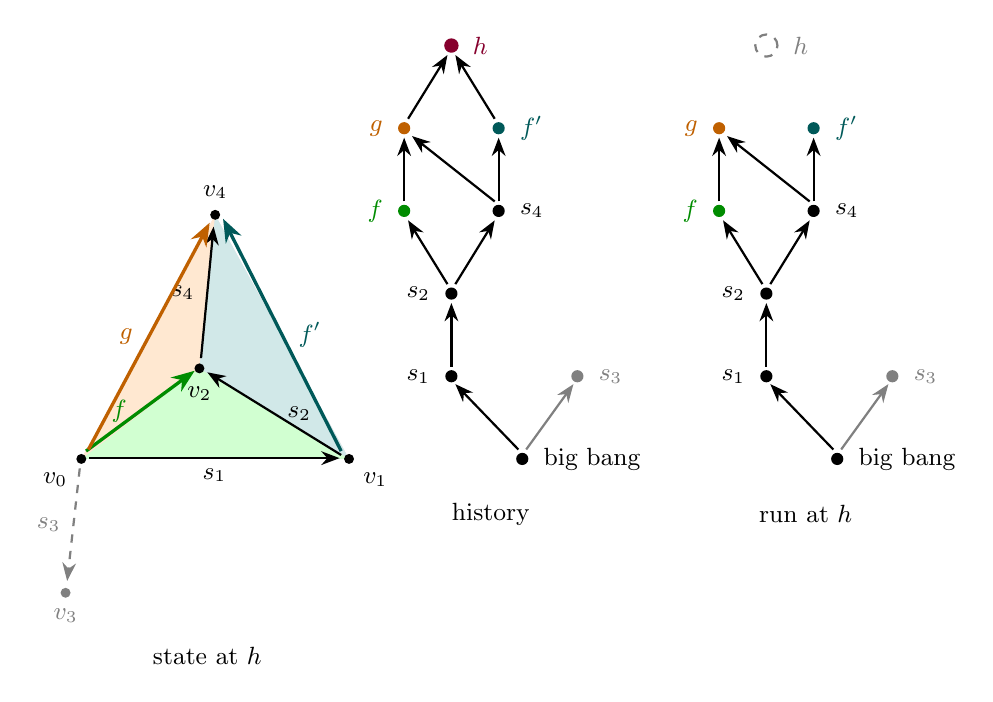
\begin{tikzpicture}[>=Stealth, thick, scale=1.0]

  % ---- left panel: the state at h ----
  % the tetrahedron on v0, v1, v2, v4, with v2 behind in projection
  % face (v0,v1,v4) supplied by h, drawn first so the others sit on top
  \fill[purple!15] (0,0) -- (3.4,0) -- (1.7,3.1) -- cycle;
  % three older 2-simplices
  \fill[green!18]  (0,0) -- (3.4,0) -- (1.5,1.15) -- cycle;
  \fill[orange!18] (0,0) -- (1.5,1.15) -- (1.7,3.1) -- cycle;
  \fill[teal!18]   (3.4,0) -- (1.5,1.15) -- (1.7,3.1) -- cycle;

  % sprout edges
  \draw[->] (0.1,0.01) -- (3.28,0.01)  node[midway, below] {\small $s_1$};
  \draw[->] (3.3,0.05) -- (1.6,1.1)    node[midway, right=1pt] {\small $s_2$};
  \draw[->] (1.52,1.28) -- (1.68,2.95) node[midway, left=1pt] {\small $s_4$};

  % composite edges
  \draw[->, green!55!black, very thick]  (0.06,0.1) -- (1.44,1.12) node[midway, left=1pt] {\small $f$};
  \draw[->, orange!75!black, very thick] (0.09,0.12) -- (1.63,3.0)  node[midway, left=2pt] {\small $g$};
  \draw[->, teal!70!black, very thick]   (3.3,0.1) -- (1.8,3.05)    node[midway, right=2pt] {\small $f'$};

  % vertices
  \fill (0,0) circle (1.8pt)     node[below left=2pt]  {\small $v_0$};
  \fill (3.4,0) circle (1.8pt)   node[below right=2pt] {\small $v_1$};
  \fill (1.5,1.15) circle (1.8pt) node[below=3pt]      {\small $v_2$};
  \fill (1.7,3.1) circle (1.8pt) node[above=2pt]       {\small $v_4$};

  % v3 is outside the state at h
  \fill[gray] (-0.2,-1.7) circle (1.8pt) node[below=2pt, gray] {\small $v_3$};
  \draw[->, gray, dashed] (-0.02,-0.12) -- (-0.18,-1.55) node[midway, left=1pt, gray] {\small $s_3$};

  \node at (1.6,-2.5) {\small state at $h$};

  % ---- middle panel: the history ----
  \begin{scope}[xshift=5.6cm]
    \fill (0,0) circle (2.2pt)                node[right=4pt] {\small big bang};
    \fill (-0.9,1.05) circle (2.2pt)          node[left=4pt]  {\small $s_1$};
    \fill[gray] (0.7,1.05) circle (2.2pt)     node[right=4pt, gray] {\small $s_3$};
    \fill (-0.9,2.1) circle (2.2pt)           node[left=4pt]  {\small $s_2$};
    \fill[green!55!black] (-1.5,3.15) circle (2.2pt) node[left=4pt]  {\small $f$};
    \fill (-0.3,3.15) circle (2.2pt)          node[right=4pt] {\small $s_4$};
    \fill[orange!75!black] (-1.5,4.2) circle (2.2pt) node[left=4pt]  {\small $g$};
    \fill[teal!70!black] (-0.3,4.2) circle (2.2pt)  node[right=4pt] {\small $f'$};
    \fill[purple!70!black] (-0.9,5.25) circle (2.6pt) node[right=4pt] {\small $h$};

    \draw[->] (-0.05,0.12) -- (-0.85,0.95);
    \draw[->, gray] (0.05,0.12) -- (0.65,0.95);
    \draw[->] (-0.9,1.17) -- (-0.9,1.98);
    \draw[->] (-0.95,2.22) -- (-1.45,3.03);
    \draw[->] (-0.85,2.22) -- (-0.35,3.03);
    \draw[->] (-1.5,3.27) -- (-1.5,4.08);
    \draw[->] (-0.35,3.27) -- (-1.4,4.1);
    \draw[->] (-0.3,3.27) -- (-0.3,4.08);
    \draw[->] (-1.45,4.32) -- (-0.95,5.13);
    \draw[->] (-0.35,4.32) -- (-0.85,5.13);

    \node at (-0.4,-0.7) {\small history};
  \end{scope}

  % ---- right panel: the run at h ----
  \begin{scope}[xshift=9.6cm]
    \fill (0,0) circle (2.2pt)                node[right=4pt] {\small big bang};
    \fill (-0.9,1.05) circle (2.2pt)          node[left=4pt]  {\small $s_1$};
    \fill[gray] (0.7,1.05) circle (2.2pt)     node[right=4pt, gray] {\small $s_3$};
    \fill (-0.9,2.1) circle (2.2pt)           node[left=4pt]  {\small $s_2$};
    \fill[green!55!black] (-1.5,3.15) circle (2.2pt) node[left=4pt]  {\small $f$};
    \fill (-0.3,3.15) circle (2.2pt)          node[right=4pt] {\small $s_4$};
    \fill[orange!75!black] (-1.5,4.2) circle (2.2pt) node[left=4pt]  {\small $g$};
    \fill[teal!70!black] (-0.3,4.2) circle (2.2pt)  node[right=4pt] {\small $f'$};

    % h is forgotten by the run
    \draw[gray, dashed] (-0.9,5.25) circle (4pt);
    \node[gray, right=6pt] at (-0.9,5.25) {\small $h$};

    \draw[->] (-0.05,0.12) -- (-0.85,0.95);
    \draw[->, gray] (0.05,0.12) -- (0.65,0.95);
    \draw[->] (-0.9,1.17) -- (-0.9,1.98);
    \draw[->] (-0.95,2.22) -- (-1.45,3.03);
    \draw[->] (-0.85,2.22) -- (-0.35,3.03);
    \draw[->] (-1.5,3.27) -- (-1.5,4.08);
    \draw[->] (-0.35,3.27) -- (-1.4,4.1);
    \draw[->] (-0.3,3.27) -- (-0.3,4.08);

    \node at (-0.4,-0.7) {\small run at $h$};
  \end{scope}

\end{tikzpicture}

  \caption{Example~\ref{ex:run}.
  Left: the state at $h$, the simplicial set itself, with sprout edges plain and the three composites colored by the fill that supplied them. The face $(v_0, v_1, v_4)$ (purple) and the solid tetrahedron come from $h$.
  Middle: the history, with $h$ (purple) a dimension-three fill sitting above the fills it depends on.
  Right: the run at $h$, the same order with $h$ forgotten, since $h$ adds no edge.
  The history remembers every event, the run drops the higher fill, and the state drops the order and the labels.}
  \label{fig:examplerun}
\end{figure}

\begin{lemma}[Exchange of order]
\label{lem:exchange}
Let $X$ be a simplicial set and let $a$ and $b$ be two events whose matches both factor through $X$.
Then $a$ and $b$ can be applied in either order, and the two resulting simplicial sets are canonically isomorphic.
\end{lemma}

\begin{proof}
Pushouts of monomorphisms in $\sset$ are monomorphisms, so the attachment map $X \to X \cup_{F_a} A_a$ is a monomorphism, and since no simplices are deleted or re-glued, the match of $b$ persists as a map into $X \cup_{F_a} A_a$.
The pushout property used here holds because pushouts in $\sset$ are computed degree by degree, and in the category of sets the pushout of an injection along any map is an injection, which is the adhesiveness property of presheaf categories \citep{ehrig2006dpo}.
Symmetrically, $a$ can be applied after $b$:
\[
\begin{tikzcd}[column sep=small]
  & X \cup_{F_a} A_a \arrow[dr, "b"] & \\
  X \arrow[ur, "a"] \arrow[dr, "b"'] & & X_{ab} \\
  & X \cup_{F_b} A_b \arrow[ur, "a"'] &
\end{tikzcd}
\]
The two routes compute the colimit of the same diagram, formed by $X$, the two matches, and the two rules, so the resulting states $X_{ab}$ are canonically isomorphic by the pasting law for pushouts.
This is the local Church--Rosser property for non-deleting double-pushout rewriting \citep{ehrig2006dpo}.
\end{proof}

\begin{proposition}[Well-definedness of the state]
\label{prop:welldef}
The causal order on the events of a history is a partial order, and for every event $e$ the colimit in Definition~\ref{def:state} exists and agrees with the state produced by any sequential build along a linear extension of $\causalO{e}$.
\end{proposition}

\begin{proof}
There are three claims to prove:
\begin{enumerate}
  \item The causal order $\causalO{e}$ of an event $e$ is a partial order.
  \item The states $X_D$ exist for all finite downsets $D$ of $\mathcal{H}$.
  \item The state at $e$ agrees with every sequential build of $\causalO{e}$.
\end{enumerate}
We prove them in that order.

\medskip
\noindent\textbf{Claim 1: the causal order is a partial order.}
This claim is a consistency check on Definition~\ref{def:history}, not a theorem about an unordered growth process.
A history presents its events as a partially ordered set from the outset, and the third condition asks this order to be the transitive closure of $\vartriangleleft$.
What needs checking is that the condition can be met, meaning that $\vartriangleleft$ generates a strict partial order.
Recall that $b$ depends on $a$ when a maximal simplex of the spot of $b$ is created by $a$.
The spot of $b$ lies in the simplicial set built by the events strictly below $b$, so every simplex of the spot is created by an event strictly below $b$, and dependency never points upward.
The transitive closure of the dependency relation is therefore contained in the strict order of the history, and a cycle of dependencies would be a cycle in that strict order, which has none.
So the dependency relation generates a strict partial order on $\causalO{e}$, as the third condition requires.
A stronger formulation is possible, in which events are given as a bare sequence of move applications with no order posited in advance, and dependency is shown acyclic by induction on position in the sequence.
We do not develop that presentation here.

\medskip
\noindent\textbf{Claim 2: the state of a finite downset exists.}
For a finite downset $D \subseteq \mathcal{H}$ we construct the simplicial set $X_D$ by induction on $|D|$, the number of events in $D$.
The induction is an algorithm that removes one event per step.
\begin{enumerate}
  \item \emph{Base case.}
        If $D = \varnothing$, set $X_\varnothing = \varnothing$, the empty simplicial set.
  \item \emph{Inductive step.}
        Suppose $X_{D'}$ has been constructed for every downset $D'$ with $|D'| < |D|$.
        Choose a maximal element $b$ of $D$ and set $D' = D \setminus \{b\}$, which is again a downset and has one element fewer.
        Let $F_b \hookrightarrow A_b$ be the rule of $b$ and $m_b : F_b \to X_{<b}$ its match, as in Definition~\ref{def:rule}.
        Every simplex in the image of $m_b$ is created by an event strictly below $b$, and every such event lies in $D'$, so the image sits inside $X_{D'}$ with its face relations unchanged, since no move deletes or re-glues anything.
        We therefore also write $m_b$ for the map $F_b \to X_{D'}$.
        Now define $X_D$ by the pushout square
        \[
        \begin{tikzcd}
          F_b \arrow[r, hook] \arrow[d, "m_b"'] & A_b \arrow[d] \\
          X_{D'} \arrow[r]                    & X_D
        \end{tikzcd}
        \]
        which attaches the new simplices of $A_b$ to $X_{D'}$ along the spot $m_b$.
  \item \emph{Termination.}
        Each step removes one event, so the recursion reaches $\varnothing$ after exactly $|D|$ steps.
        Since $D$ is finite, this always stops.
  \item \emph{The choice of maximal element does not matter.}
        If $b_1 \neq b_2$ are both maximal in $D$, they are incomparable, and $D'' = D \setminus \{b_1, b_2\}$ is again a downset, and it contains every event strictly below $b_1$ or $b_2$.
        Both matches therefore factor through $X_{D''}$.
        By the induction hypothesis, $X_{D \setminus \{b_1\}}$ can be computed by attaching $b_2$ to $X_{D''}$, and $X_{D \setminus \{b_2\}}$ can be computed by attaching $b_1$ to $X_{D''}$.
        Lemma~\ref{lem:exchange} identifies the two routes to $X_D$, and induction on $|D|$ then shows that $X_D$ is independent of all such choices.
\end{enumerate}
Applying this to $D = \causalO{e}$ defines the state $X_e := X_{\causalO{e}}$.
The causal order $\causalO{e}$ is finite by the definition of a history, so the algorithm applies.

\medskip
\noindent\textbf{Claim 3: every sequential build agrees with the colimit.}
Fix a linear extension of $\causalO{e}$ and build the state event by event along it.
\begin{enumerate}
  \item Any two linear extensions of a finite poset are connected by a sequence of adjacent transpositions of incomparable elements.
        If $a$ and $b$ are adjacent in the extension and incomparable in the causal order, then every event strictly below $b$ precedes $a$ in the extension, since it cannot lie between two adjacent events and cannot be $a$ itself.
        Both matches then factor through the state built before $a$, and Lemma~\ref{lem:exchange} shows that swapping the two events does not change the result.
        So all sequential builds of $\causalO{e}$ agree.
  \item The chain of downsets
        \[
          \varnothing \subsetneq \{e_1\} \subsetneq \{e_1, e_2\} \subsetneq \dots \subsetneq \causalO{e}
        \]
        built along a linear extension is final in the poset of downsets of $\causalO{e}$, meaning that every downset is contained in some member of the chain, and the members are nested.
        Hence the colimit over the downset diagram equals the colimit along the chain.
  \item The colimit along the chain is the iterated pushout, which is exactly what the sequential build computes.
\end{enumerate}
Hence every sequential build produces the state $X_e$ of Definition~\ref{def:state}.
\end{proof}

\subsection{Branching, reversal closure, and the homotopy ledger}
\label{sec:kfold}

This subsection extends the framework of Definition~\ref{def:moves}.
The base framework is contractible at every event, and Corollary~\ref{cor:nocommonfuture} is the geometric face of that commitment: reachability is an ancestor relation of a rooted tree, so no two incomparable vertices ever acquire a common future, and no place for a spatial separation exists.
This section admits the smallest family of moves that changes this, audits exactly what each admission costs, and proves the accounting identity that governs all of them.

Three observations organize what follows.
First, every fill is a pushout of an inner horn inclusion, hence a pushout of an anodyne extension; anodyne extensions are closed under pushout and are trivial cofibrations, so \textbf{a fill in any dimension is a weak homotopy equivalence and never alters a homotopy invariant of the state}.
All homotopy is therefore minted by creation moves alone.
Second, the move set as it stands is not closed under the opposite construction $(-)^{\mathrm{op}}$, which reverses the order of every simplex: $\mathrm{op}$ preserves colimits and monomorphisms, fixes $\Delta^0$, and carries $\Lambda^1_0 \hookrightarrow \Delta^1$ to $\Lambda^1_1 \hookrightarrow \Delta^1$, so a history built under one move set has its mirror built under the other, and the two sets must be admitted together for either mirror to be a state of the same framework.
Third, the obstruction itself has a precise source: every vertex receives exactly one edge from the creation event that made it, so common pasts are free while common futures across incomparable vertices are impossible.
Any repair must let a fresh vertex receive edges from more than one existing vertex, and reversal closure forces the dual move alongside it.

\begin{definition}[$k$-fold sprout]
\label{def:kfold}
For $k \geq 1$ let $E_k$ be the simplicial set consisting of $k$ vertices and nothing else, and let $C_k$ be the join of $E_k$ with a single vertex, that is, $k+1$ vertices together with one edge from each vertex of $E_k$ to the new one.
The \textbf{$k$-fold sprout} is the pushout along $E_k \hookrightarrow C_k$.
A match is an injective map $E_k \to X_{<e}$, so it picks $k$ distinct existing vertices; since $\operatorname{Aut}(E_k) = S_k$ acts on the inclusion by automorphisms, the ordering of the chosen vertices is not part of the data and the match may be read as an unordered $k$-element subset.
The move attaches a fresh vertex together with one edge into it from each matched vertex, giving it those $k$ parents.
The sprout of Definition~\ref{def:moves} is the case $k = 1$.
\end{definition}

\begin{definition}[Co-sprout]
\label{def:cosprout}
The \textbf{$k$-fold co-sprout} is the pushout along the opposite inclusion $(C_k)^{\mathrm{op}}$: it attaches a fresh vertex carrying one edge out of it into each of $k$ distinct existing vertices, giving them a shared future vertex.
The one-fold co-sprout, the pushout along $\Lambda^1_1 \hookrightarrow \Delta^1$, is the horn whose admission was declined in Remark~\ref{rem:sproutishorn}.
Both families are rules in the sense of Definition~\ref{def:rule}, delete nothing, and need no global check: a freshly created vertex cannot complete a directed cycle at the moment of its creation, whatever the orientation of its edges, so Lemma~\ref{lem:acyclic} holds verbatim for the extended move set, by the proof given there.
Lemma~\ref{lem:exchange} and Proposition~\ref{prop:welldef} use only that rules are monomorphisms and that nothing is deleted or re-glued, so they hold unchanged, and Definition~\ref{def:run} stands with the run still consisting of the edge-adding events.
Lemma~\ref{lem:edges} gains one clause per family: a $k$-fold sprout or co-sprout adds exactly $k$ edges.
\end{definition}

The two families do different jobs, and the difference is the point.
$\mathrm{op}$ is an involution of $\sset$ preserving colimits and monomorphisms and fixing $\Delta^0$, so applying it to a history built under one move set yields the mirror history built under the opposite move set in the same order.
A move set is closed under reversal exactly when it contains both families, and only a closed set makes the mirror of every state a state, which is what the broken-symmetry discussion of the Introduction requires.
Geometrically, a $k$-fold sprout hands its $k$ matched vertices a common future; a co-$k$-fold hands them a common past.
Since every pair of vertices already shares the root as a common past, only the sprout family buys new spacelike structure, and the co-sprout family exists for closure.
One caution: a $k$-fold sprout at a pairwise comparable set pays every cost of branching and buys nothing, since those vertices already had common futures; the spacelike content of a move lies in whether its match spans incomparable vertices, and a rule can be constrained to that case without loss.

What the extension costs outside homotopy is limited and worth stating plainly.
Proposition~\ref{prop:tree} and Corollary~\ref{cor:nocommonfuture} fail, which is the purpose: ancestors form a directed acyclic graph rather than a chain, and Proposition~\ref{prop:zeroentropy} fails in both clauses, since a multi-vertex sprout depends on the creators of its $k$ matched vertices, which need not be comparable, so creation events themselves can carry entropy.

\begin{proposition}[The homotopy ledger]
\label{prop:ledger}
Let $e$ be an event of a history built with sprouts, co-sprouts, $k$-fold versions of both, and inner fills.
Then the state $X_e$ is connected and
\[
X_e \;\simeq\; \bigvee_{a}\; S^1 \vee \dots \vee S^1,
\qquad
\beta_1(X_e) \;=\; \sum_{a \preceq e} \bigl(k_a - 1\bigr),
\]
where the sum runs over the multi-vertex creation events $a$ below $e$, $k_a$ is the number of vertices matched by $a$, and all higher homotopy groups vanish.
In particular every fill contributes nothing, and a history under the base move set of Definition~\ref{def:moves} reads zero at every event, recovering contractibility as the zero row of the ledger rather than an additional assumption.
\end{proposition}

\begin{proof}
States remain connected by induction, since every move attaches its fresh vertices along at least one edge to the existing state.
Each creation move is the attachment of a cone $\mathrm{Cone}(E_k)$ along the discrete subspace $E_k$ of $k$ points.
For $k=1$ this is an interval attached at an endpoint, hence a weak equivalence contributing nothing.
For $k \geq 2$, the long exact sequence of the pair $(\mathrm{Cone}(E_k), E_k)$ gives $\widetilde{H}_n(\mathrm{Cone}(E_k), E_k) = 0$ for $n \neq 1$ and $\widetilde{H}_1 \cong \mathbb{Z}^{k-1}$; equivalently, van Kampen for groupoids exhibits the new fundamental group as a free product with a free group of rank $k-1$, leaving all higher homotopy groups unchanged.
Fills are pushouts of inner horn inclusions, hence of anodyne extensions; anodyne extensions are closed under pushout and are trivial cofibrations, so every fill is a weak equivalence and contributes no entry.
Summing the contributions of the creation events along any linear extension of $\causalO{e}$ gives the identity, with the wedge decomposition assembled one circle at a time.
\end{proof}

\begin{corollary}[Contractibility as bookkeeping]
\label{cor:ledgerzero}
A history conserves the homotopy type of a point if and only if every creation event matches exactly one vertex.
Every departure costs $k_a - 1$ circles at event $a$, minted once and never removed, since no later move alters any homotopy invariant.
\end{corollary}

\begin{remark}[The universe as a wedge of circles]
\label{rem:wedge}
Under the base move set the ledger is identically zero and Remark~\ref{rem:contractible} applies in full strength: there are no topological observables at all.
Under branching, the entire homotopy information of every state is the non-negative integer $\beta_1(X_e)$, which is monotone along the causal order, visible to the run since multi-vertex sprouts add edges, and insensitive to everything else the history records.
All deeper structure lives in the directed homotopy type of the limit quasicategory, not in the homotopy type of the states.
\end{remark}

\begin{proposition}[Diamonds require branching]
\label{prop:diamondbranching}
In the base framework of Definition~\ref{def:moves}, two vertices have a common future only if they are comparable.
More generally, under any move set in which every composite edge runs parallel to an existing directed path: if $u$ and $w$ are incomparable vertices and some vertex is reachable from both, then some creation event matched a set containing two incomparable vertices.
\end{proposition}

\begin{proof}
Let $u$ and $w$ be incomparable, and let $m$ be minimal among vertices reachable from both, where paths of length zero are allowed.
Every directed path into $m$ ends in a creation edge into $m$: composites run parallel to earlier directed paths, so tracing any path backwards past its composite edges terminates at a creation edge.
Hence $u$ reaches $m$ through some creation parent $p_1$ of $m$ and $w$ through some creation parent $p_2$.
If all creation parents of $m$ were pairwise comparable, then relabelling gives $p_1$ reachable-to $p_2$ through the parents' own edges, so both $u$ and $w$ reach $p_2$, and $p_2$ is an older vertex than $m$, contradicting minimality of $m$.
So $m$ has two incomparable creation parents, and these are distinct matched vertices of the creating event.
\end{proof}

\begin{corollary}[No branching, no diamonds]
\label{cor:diamondcircle}
If every creation match is contained in a single ancestor chain, every pair of vertices with a common future is comparable, and no causal diamond ever forms.
Conversely, a $k$-fold sprout at an incomparable pair immediately produces a diamond: its fresh vertex is a common future of the pair, and their common ancestor chain provides a common past.
\end{corollary}

Combining the two halves: a diamond forces a branching event, the branching event pays $k-1$ circles by Proposition~\ref{prop:ledger}, and the payment is permanent.
Within this move idiom, spacelike separation and nontrivial topology are the same expenditure seen from two sides.
The converse fails, and the failure is diagnostic: a $k$-fold sprout at a comparable pair pays a full circle and produces no diamond, and the residual loop there is a doubled-edge artifact, a composite running parallel to a creation edge with no cell distinguishing them.
Topology tracks the connectivity structure of matches; diamonds track their incomparability.
Whether a rule can be found that branches only where diamonds result is a question about the constraint set of the inference problem, and Section~\ref{sec:background} does not answer it here.

\begin{remark}[The limit has genuinely distinct parallel paths]
\label{rem:limitpaths}
Fairness asks that every inner horn that exists be filled eventually, and nothing in this subsection conflicts with it: a horn spanning an incomparable pair never exists, because $\Delta^3$ needs all six edges of its tetrahedron and no move ever supplies an edge between incomparable vertices, so there is no unmet obligation.
What fails instead is uniqueness of composition.
At a diamond the two routes from past to future yield two composite edges from $p$ to $m$, supplied by fills of different horns, and no simplex of the state ever identifies them, so the limit quasicategory contains genuinely distinct parallel morphisms between the same endpoints.
This is Proposition~\ref{prop:ledger} restated categorically: the wedge summands are precisely the non-homotopic pairs of parallel composites.
The classical zero-information limit in which every filler is unique is thus available exactly when the ledger reads zero.
\end{remark}

One further point is worth recording.
A move that attaches a fresh element to the future of a chosen set of existing elements is exactly the growth step of the classical sequential growth models of \citet{rideout2000csg}, in which the fresh element is added to the future of an arbitrary subset of the existing causal set, and in which manifold-like causal sets are at least reachable.
Adopting Definitions~\ref{def:kfold} and~\ref{def:cosprout} therefore puts the framework in a setting where the recovery of a geometry is a live question rather than one already closed by Corollary~\ref{cor:nocommonfuture}.
It also makes the overlap with that literature substantial, so the novelty claims in Section~\ref{sec:background} have to be written against it.

\gap{Three decisions remain before the inference problem is posed. First, fix the move set: the base set of Definition~\ref{def:moves} keeps contractibility and loses diamonds outright; adding the $k$-fold sprout alone leaves the move set open under $(-)^{\mathrm{op}}$, so reversal closure argues for admitting the co-sprout family alongside, per Definition~\ref{def:cosprout}. Second, decide whether the rule constrains creation matches to span incomparable sets, which is the efficient regime identified after Corollary~\ref{cor:diamondcircle}. Third, Remark~\ref{rem:notafunctionofrun} has sharpened rather than resolved: the run sees exactly the integer $\beta_1$ of Proposition~\ref{prop:ledger}, so the geometric trace knows the topology of the deep structure but not its entropy, and whichever observable pairs with entropy in an area law must see more of the run than the one-skeleton currently exposes. The exhaustiveness of the case analysis --- arrow, contractibility, diamonds, choose two --- remains open beyond move sets satisfying the parallel-path condition of Proposition~\ref{prop:diamondbranching}.}

\section{Finite-model predictions}
\label{sec:toyresults}

The four-history model gives explicit calculations with which to check the
framework. They are standard quantum predictions under the assumptions of
Section~\ref{sec:twopath}, not new experimental evidence or a derivation of
quantum mechanics.

\subsection{Output interference}

The output partition is decoherent for every $\phi$ and $\gamma$, since
the kernel has no entries joining different output labels. Its probabilities
are
\begin{equation}
  p(A_0)=\frac{1+\gamma\cos\phi}{2},\qquad
  p(A_1)=\frac{1-\gamma\cos\phi}{2}.
  \label{eq:toyfringes}
\end{equation}
At $\gamma=1$ and $\phi=0$, output $1$ has zero probability even though
both histories ending there have nonzero amplitudes. The exclusion is due
to cancellation, not inadmissibility. At $\gamma=0$, the probabilities are
both $1/2$ and phase dependence disappears.

\begin{table}[ht]
  \centering
  \begin{tabular}{ccccc}
    \hline
    $\gamma$ & $\phi$ & $p(A_0)$ & $p(A_1)$ & Auxiliary route record\\
    \hline
    $1$ & $0$ & $1$ & $0$ & Identical states\\
    $1$ & $\pi/2$ & $1/2$ & $1/2$ & Identical states\\
    $1$ & $\pi$ & $0$ & $1$ & Identical states\\
    $0$ & Any & $1/2$ & $1/2$ & Orthogonal states\\
    \hline
  \end{tabular}
  \caption{Exact predictions of the specified finite model. Admissibility
  and the number of histories are unchanged in every row.}
  \label{tab:toyoutputs}
\end{table}

The output-$0$ fringe visibility, defined by sweeping $\phi$ at fixed
$\gamma$, is
\[
  V=\frac{p_{\max}(A_0)-p_{\min}(A_0)}
          {p_{\max}(A_0)+p_{\min}(A_0)}=\gamma.
\]
The connection between records and interference is therefore quantitative.
It follows from the supplied inner product on record states, not from
the number or connectivity of the histories.

\subsection{Which alternatives decohere}

The route partition is also decoherent, with $p(C_0)=p(C_1)=1/2$.
However, the common refinement of the route and output partitions is the
singleton partition of $\Omega$. For its distinct histories ending at the
same output,
\[
  \left|D(\{H_{0d}\},\{H_{1d}\})\right|=\frac{\gamma}{4}.
\]
The refinement is exactly decoherent, in the sense defined here, only
when $\gamma=0$. Separately admissible probability questions therefore
need not combine into a finer decoherent question.

At $\gamma=1$, the route partition decoheres even though the auxiliary
states contain no route record. Thus decoherence of a partition is not by
itself a construction of a physical recorder. At $\gamma=0$, the auxiliary
states distinguish the routes and the refined probabilities are $1/4$
for each history. Labels that merely name alternatives and states that
record alternatives do different work in the model.

Replacing $K$ by its diagonal gives $p_{\mathrm{diag}}(A_d)=1/2$ at every
phase. The discrepancy at the outputs, in total variation distance, is
\begin{equation}
  \frac12\sum_{d=0}^1
    |p(A_d)-p_{\mathrm{diag}}(A_d)|
    =\frac{\gamma|\cos\phi|}{2}\leq\frac{\gamma}{2}.
  \label{eq:classicalerror}
\end{equation}
This is an error bound for this specified output question. It is not a
bound for every possible measurement. A small discrepancy at one phase
does not establish decoherence of the refined family.

\subsection{Entropy depends on the record question}

Write $h(x)=-x\log x-(1-x)\log(1-x)$, with $0\log0=0$. The Shannon
entropy of the detector outcomes is
\[
  S_{\mathrm{out}}=h\!\left(\frac{1+\gamma\cos\phi}{2}\right).
\]
In the supplied quantum description the reduced auxiliary record state is
\[
  \rho_{\mathrm{rec}}
    =\frac12\bigl(|r_0\rangle\langle r_0|
                 +|r_1\rangle\langle r_1|\bigr),
\]
with von Neumann entropy
\[
  S_{\mathrm{rec}}=h\!\left(\frac{1+\gamma}{2}\right).
\]
At $\gamma=1$ and $\phi=\pi/2$, the output entropy is $\log2$ while the
record entropy is zero. The same allowed histories also give zero output
entropy at $\gamma=1$ and $\phi=0$. Counting the four histories would give
$\log4$ in both cases. These are different quantities, not competing
calculations of one universal entropy. None is an area or a horizon entropy.

\subsection{A controlled sensitivity calculation}

For the output distributions at parameter settings $(\gamma,\phi)$ and
$(\widetilde\gamma,\widetilde\phi)$, the total variation distance is
\begin{equation}
  \frac12\sum_{d=0}^1|p(A_d)-\widetilde p(A_d)|
   =\frac12|\gamma\cos\phi-\widetilde\gamma\cos\widetilde\phi|
   \leq\frac12\bigl(|\gamma-\widetilde\gamma|
                      +|\phi-\widetilde\phi|\bigr).
  \label{eq:toysensitivity}
\end{equation}
Here the phases are represented by real numbers. This is a finite
sensitivity bound for two specified weighting parameters and one output
partition. It does not establish universality under changes to the
relational signature, stability of a spacetime, or persistence under an
internal clock.

\section{What the model tests}
\label{sec:discussion}

The finite example separates three kinds of restriction that a physical
proposal must not confuse. Admissibility excludes structures that are not
in $\Omega$. Interference can give zero probability to an alternative
assembled from allowed histories. Decoherence determines when those
alternatives can be treated with additive probabilities. None of these
restrictions substitutes for the other two.

\subsection{The weighting must constrain predictions}

The same possibility space supports every row of
Table~\ref{tab:toyoutputs}. Its unlabelled topology is unchanged as well.
Thus admissibility and topology do not select the predictions in this
example. This is not an argument that structure could never constrain a
weighting. It identifies information that the particular relational
structure does not contain.

Allowing an arbitrary positive kernel for each experimental setting would
leave the proposal without a predictive weighting law. Even diagonal
kernels allow arbitrary probability assignments to the four histories.
The example obtains a restriction by holding the mixing operations fixed
and prescribing how phase and record overlap enter their composition.
Explaining that prescription structurally would be a further result.
Renaming its matrices as local rules would not be such an explanation.

The finite example also distinguishes quantum interference from an
ontological assertion that one history is randomly selected. It calculates
probabilities for outputs, but supplies no mechanism selecting one outcome
and does not decide between interpretations of quantum mechanics.

\subsection{Failure criteria}

For the supplied two-path prescription, the phase dependence must obey
Equation~\ref{eq:toyfringes}, visibility must agree with the record overlap,
and the diagonal approximation must have the discrepancy in
Equation~\ref{eq:classicalerror}. A comparison requires independently
specified preparation, mixing operations, record coupling, and detector
conditions. Adjusting these separately for every observed probability
would not test the prescription. Losses would require additional
alternatives or an explicitly conditioned experiment.

These are tests of a standard quantum toy model, not distinctive predictions
of a new spacetime theory. Nor does a two-output interference curve by
itself rule out all classical models with setting-dependent probabilities.
The broader target still requires compatible predictions across different
measurement operations, including genuinely quantum correlations.

A spacetime candidate would face additional failure criteria. Its record
predictions must survive the proposed removal of the regulator. The same
microscopic prescription must account for both geometric and matter
observations without independent fits. Any claimed robustness must persist
over stated changes to microscopic structure, rather than only over the
two continuous parameters used here. Failure on any of these conditions
would reject that candidate, not be repaired by the generality of the
framework.

\subsection{What remains unexplained}

The example shows how a weighted history description can retain
interference while allowing particular coarse records to have ordinary
probabilities. It also shows where the quantum content was supplied.
There is no derived metric, physical clock, gravitational dynamics,
quantum field theory, or stable large-scale geometry in the calculation.
The mixing order is imposed, and the auxiliary record space lies outside
the bare relational description.

The remaining structural problem is therefore specific. A candidate must
explain a restricted composition and weighting prescription, give an
internal account of records, and identify a regime with a common geometric
and quantum description. The calculations here provide checks that such
a candidate should pass. They do not establish that a suitable candidate
exists.


\bibliographystyle{plainnat}
\bibliography{bibliography/references}

\end{document}
